\section*{7}

\begin{enumerate}[label=\alph*)]
    \item
        对于该优化问题, 构造Lagrange函数
        \begin{equation*}
            \mathcal{L}(\bm{x},\bm{\lambda})=f(\bm{x})+\sum_{i=1}^4\lambda_ig_i(\bm{x}),
        \end{equation*}
        其中
        \begin{align*}
            &f(\bm{x})=(x_1-3)^2+(x_2-2)^2, \\
            &g_1(\bm{x})=x_1^2+x_2^2-5, \\
            &g_2(\bm{x})=x_1+2x_2-4, \\
            &g_3(\bm{x})=-x_1, \\
            &g_4(\bm{x})=-x_2, \\
        \end{align*}
        则该优化问题的KKT条件为
        \begin{equation*}
            \begin{cases}
                g_i(\bm{x})\leq0, &i=1,2,3,4, \\
                \lambda_i\geq0, &i=1,2,3,4, \\
                \lambda_ig_i(\bm{x})=0, &i=1,2,3,4, \\
                \nabla_{\bm{x}}\mathcal{L}(\bm{x},\bm{\lambda})=\bm{0}, &i=1,2,3,4.
            \end{cases}
        \end{equation*}

    \item 在点$(0,0)^\mathrm{T}$处, 有$\lambda_1,\lambda_2=0$, $\lambda_3=-6$, $\lambda_4=-4$, 不满足KKT条件, 因此不是KKT点.
    \item 在点$(2,1)^\mathrm{T}$处, 有$\lambda_1=\frac{1}{3}, \lambda_2=\frac{2}{3}, \lambda_3,\lambda_4=0$, 满足KKT条件, 因此是KKT点.
    \item
        如\cref{figure:7d}, 在点$(0,0)^\mathrm{T}$处, 起作用约束条件的梯度与下降方向的夹角大于$\frac{\pi}{2}$, 不满足要求, 因此不是KKT点.
        在点$(2,1)^\mathrm{T}$处起作用约束条件的梯度与下降方向小于$\frac{\pi}{2}$, 满足要求, 因此是KKT点.
        \begin{figure}[ht]
            \centering
            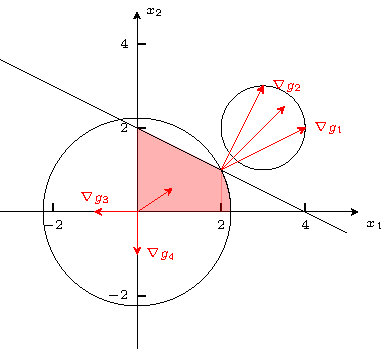
\includegraphics[scale = 1.2]{figures/7d.pdf}
            \caption{优化问题的几何示意图}
            \label{figure:7d}
        \end{figure}
\end{enumerate}
